\documentclass{amsart}
%DIF LATEXDIFF DIFFERENCE FILE
%DIF DEL report.tex     Fri Apr 23 22:31:01 2021
%DIF ADD report11.tex   Fri Apr 23 22:30:35 2021
\synctex=1
%DIF 3-6c3
%DIF < 
%DIF < %=================================================================
%DIF < % 
%DIF < \newcount\DraftStatus  % 0 suppresses notes to selves in text
%DIF -------
\newcount\DraftStatus   %DIF > 
%DIF -------
\DraftStatus=1   % TODO: set to 0 for final version
%DIF 8-10d5
%DIF < %=================================================================
%DIF < 
%DIF < %=================================================================
%DIF -------
\usepackage{comment}
%DIF 12-13d6
%DIF < %=================================================================
%DIF < %
%DIF -------
\includecomment{JournalOnly}  
\includecomment{ConferenceOnly}  
\includecomment{TulipStyle}
%DIF 17d9
%DIF < %
%DIF -------
%=================================================================
%DIF 19a10
%================================================================= %DIF > 
%DIF -------
%=================================================================
% gitlatexdiff
%
%  https://gitlab.com/git-latexdiff/git-latexdiff
%=================================================================
%  git latexdiff HEAD  HEAD~5 --main templatex.tex
%  git latexdiff HEAD~1  --main templatex.tex
%  View pdf to see difference
%
%=================================================================
%
% Todo Notes for marginal comments
% 
%\newcount\DraftStatus  % 0 suppresses notes to selves in text
%\DraftStatus=1   % TODO: set to 0 for final version
\ifnum\DraftStatus=1
	\usepackage[draft,colorinlistoftodos,color=orange!30]{todonotes}
\else
	\usepackage[disable,colorinlistoftodos,color=blue!30]{todonotes}
\fi 
%\usepackage[disable]{todonotes} % notes not showed
%\usepackage[draft]{todonotes}   % notes showed
%
\makeatletter
 \providecommand\@dotsep{5}
 \def\listtodoname{List of Todos}
 \def\listoftodos{\@starttoc{tdo}\listtodoname}
 \makeatother
%
%=================================================================
%
\usepackage{color}
\newcommand{\draftnote}[3]{ 
	\todo[author=#2,color=#1!30,size=\footnotesize]{\textsf{#3}}	}
% TODO: add yourself here:
%
\newcommand{\gangli}[1]{\draftnote{blue}{GLi:}{#1}}
\newcommand{\qwu}[1]{\draftnote{red}{QWu:}{#1}}
\newcommand{\gliMarker}
	{\todo[author=GLi,size=\tiny,inline,color=blue!40]
	{Gang Li has worked up to here.}}
\newcommand{\qwuMarker}
	{\todo[author=QWu,size=\tiny,inline,color=red!40]
	{Qiong Wu has worked up to here.}}
%=================================================================

%=================================================================
%
% general packages
%  https://en.wikibooks.org/wiki/Category:Book:LaTeX
%  https://en.wikibooks.org/wiki/LaTeX/Package_Reference
%
%=================================================================
\usepackage{graphicx}
\usepackage{algorithm}
\usepackage{algorithmic}
\usepackage{breqn}
\usepackage{subcaption}
\usepackage{multirow}
\usepackage{psfrag}
\usepackage{url}
\usepackage{hyperref}
%\usepackage[colorlinks]{hyperref}
%\usepackage{cite}
\usepackage{cleveref}
\usepackage{booktabs}
\usepackage{rotating}
\usepackage{colortbl}
\usepackage{paralist}
%\usepackage{geometry}
\usepackage{epstopdf}
\usepackage{nag}
\usepackage{microtype}
\usepackage{siunitx}
\usepackage{nicefrac}
\usepackage{breakurl}
\usepackage{fontawesome}
\usepackage{xcolor}
\usepackage{multicol}
\usepackage{wrapfig}
\usepackage{todonotes}
\usepackage{tablefootnote}
\usepackage{threeparttable}
% for random text
\usepackage{lipsum}
\usepackage[english]{babel}
\usepackage[pangram]{blindtext}
% for tikz figures
\usepackage{tikz}
\usetikzlibrary{fit,positioning,arrows.meta,shapes,arrows}
%\tikzset{neuron/.style={circle,thick,fill=black!25,minimum size=17pt,inner sep=0pt},
%	input neuron/.style={neuron, draw,thick, fill=gray!30},
%	hidden neuron/.style={neuron,fill=white,draw},
%	hoz/.style={rotate=-90}}
%
%=================================================================



\begin{TulipStyle}
\usepackage[numbers]{natbib}
%=================================================================
%
% Version control information
%
%=================================================================
\usepackage{gitinfo2}
%=================================================================
\usepackage{fancyhdr}
\pagestyle{fancy}
\fancyhead{} % clear all header fields
\fancyhead[RO,LE]{\textsl{\rightmark}}
\fancyhead[LO,RE]{\ensuremath{\Rightarrow}
		\textbf{\textbf{[CONFIDENTIAL]}}\ensuremath{\Leftarrow}}
\fancyhead[CO,CE]{}
%=================================================================
\fancyfoot{} % clear all footer fields
\fancyfoot[CE,CO]{\textbf{\thepage}} 
\fancyfoot[LO,LE]{
\includegraphics[height=.9\headheight]{logos/tulip-logo.eps}
		\gitVtagn-\gitBranch\ (\gitCommitterDate)}
\fancyfoot[RO,RE]{Committed by: \textsl{\gitCommitterName}}

\setlength{\headheight}{12pt}
\renewcommand{\headrulewidth}{0.4pt}
\renewcommand{\footrulewidth}{0.4pt}
%=================================================================


%=================================================================
% for math notations
% ----------------------------------------------------------------
\usepackage{mathtools}
\usepackage{amsthm}
%
% THEOREMS -------------------------------------------------------
%
\newtheorem{thm}{Theorem}[section]
\newtheorem{cor}[thm]{Corollary}
\newtheorem{lem}[thm]{Lemma}
\newtheorem{prop}[thm]{Proposition}
\theoremstyle{definition}
\newtheorem{defn}[thm]{Definition}
\theoremstyle{remark}
\newtheorem{rem}[thm]{Remark}
\numberwithin{equation}{section}
% MATH -----------------------------------------------------------
\newcommand{\norm}[1]{\left\Vert#1\right\Vert}
\newcommand{\abs}[1]{\left\vert#1\right\vert}
\newcommand{\set}[1]{\left\{#1\right\}}
\newcommand{\Real}{\mathbb R}
\newcommand{\eps}{\varepsilon}
\newcommand{\To}{\longrightarrow}
\newcommand{\BX}{\mathbf{B}(X)}
% ----------------------------------------------------------------
\newcommand{\I}{{\cal I}}
\newcommand{\Id}{{\cal I} }
\newcommand{\Dc}{{\cal D}}
\newcommand{\J}{{\cal J}}
\newcommand{\Dn}{{\cal D}_n}
\newcommand{\Dd}{{\cal D}_n }
\renewcommand{\P}{{\cal P}}
\newcommand{\Nu}{{\cal N} }
\newcommand{\B}{{\cal B}}
\newcommand{\Bf}{{\bf B}}
\newcommand{\Y}{{\bf Y}}
\newcommand{\A}{{\cal A}}
% ----------------------------------------------------------------
\newcommand{\V}{{\cal V}}
\newcommand{\M}{{\cal M}}
\newcommand{\F}{{\cal F}}
\newcommand{\Fd}{{\cal F}}
\newcommand{\BF}{{\cal BF}_n}
\newcommand{\BFd}{{\cal BF}_n}
\newcommand{\TF}{{\cal TF}_n}
\newcommand{\TFd}{{\cal TF}_n}
%\newcommand{\G}{{\cal G}}
\newcommand{\X}{{\cal X}}
\newcommand{\E}{{\cal E}}
\newcommand{\K}{{\cal K}}
\newcommand{\T}{{\cal T}_n}
\renewcommand{\H}{{\cal H}}
% ----------------------------------------------------------------
\newtheorem{Remark}{Remark}
\newtheorem{proposition}{Proposition}
\newtheorem{theorem}{Theorem}
\newtheorem{lemma}{Lemma}
\newtheorem{corollary}{Corollary}
\newtheorem{example}{Example}
\newtheorem{definition}{Definition}
\newtheorem{Algorithms}{Algorithm}
% ----------------------------------------------------------------
\newcommand{\bu}{{\mathbf 1} }
\newcommand{\bo}{{\mathbf 0} }
\newcommand{\N}{\mbox{{\sl l}}\!\mbox{{\sl N}}}
% ----------------------------------------------------------------
\def\uint{[0,1]}
\def\proof{{\scshape Proof}. \ignorespaces}
\def\endproof{{\hfill \vbox{\hrule\hbox{%
   \vrule height1.3ex\hskip1.0ex\vrule}\hrule
  }}\par}
%
%=================================================================

\hypersetup
{
    pdfauthor={\gitAuthorName},
    pdfsubject={TULIP Lab},
    pdftitle={},
    pdfkeywords={TULIP Lab, Data Science},
%	bookmarks=true,  
}

\end{TulipStyle}


%DIF 20-21d12
%DIF < 
%DIF < 
%DIF -------
%=================================================================
%DIF < %
%DIF PREAMBLE EXTENSION ADDED BY LATEXDIFF
%DIF UNDERLINE PREAMBLE %DIF PREAMBLE
\RequirePackage[normalem]{ulem} %DIF PREAMBLE
\RequirePackage{color}\definecolor{RED}{rgb}{1,0,0}\definecolor{BLUE}{rgb}{0,0,1} %DIF PREAMBLE
\providecommand{\DIFadd}[1]{{\protect\color{blue}\uwave{#1}}} %DIF PREAMBLE
\providecommand{\DIFdel}[1]{{\protect\color{red}\sout{#1}}}                      %DIF PREAMBLE
%DIF SAFE PREAMBLE %DIF PREAMBLE
\providecommand{\DIFaddbegin}{} %DIF PREAMBLE
\providecommand{\DIFaddend}{} %DIF PREAMBLE
\providecommand{\DIFdelbegin}{} %DIF PREAMBLE
\providecommand{\DIFdelend}{} %DIF PREAMBLE
\providecommand{\DIFmodbegin}{} %DIF PREAMBLE
\providecommand{\DIFmodend}{} %DIF PREAMBLE
%DIF FLOATSAFE PREAMBLE %DIF PREAMBLE
\providecommand{\DIFaddFL}[1]{\DIFadd{#1}} %DIF PREAMBLE
\providecommand{\DIFdelFL}[1]{\DIFdel{#1}} %DIF PREAMBLE
\providecommand{\DIFaddbeginFL}{} %DIF PREAMBLE
\providecommand{\DIFaddendFL}{} %DIF PREAMBLE
\providecommand{\DIFdelbeginFL}{} %DIF PREAMBLE
\providecommand{\DIFdelendFL}{} %DIF PREAMBLE
%DIF LISTINGS PREAMBLE %DIF PREAMBLE
\RequirePackage{listings} %DIF PREAMBLE
\RequirePackage{color} %DIF PREAMBLE
\lstdefinelanguage{DIFcode}{ %DIF PREAMBLE
%DIF DIFCODE_UNDERLINE %DIF PREAMBLE
  moredelim=[il][\color{red}\sout]{\%DIF\ <\ }, %DIF PREAMBLE
  moredelim=[il][\color{blue}\uwave]{\%DIF\ >\ } %DIF PREAMBLE
} %DIF PREAMBLE
\lstdefinestyle{DIFverbatimstyle}{ %DIF PREAMBLE
	language=DIFcode, %DIF PREAMBLE
	basicstyle=\ttfamily, %DIF PREAMBLE
	columns=fullflexible, %DIF PREAMBLE
	keepspaces=true %DIF PREAMBLE
} %DIF PREAMBLE
\lstnewenvironment{DIFverbatim}{\lstset{style=DIFverbatimstyle}}{} %DIF PREAMBLE
\lstnewenvironment{DIFverbatim*}{\lstset{style=DIFverbatimstyle,showspaces=true}}{} %DIF PREAMBLE
%DIF END PREAMBLE EXTENSION ADDED BY LATEXDIFF

\begin{document}
\DIFaddbegin \title[Group 00]{\DIFadd{The end of 00 Report}}\DIFaddend %
\DIFaddbegin \author{\DIFadd{Sarah Sun}}
\address[A.~1]{School of business and law,\\ 
Deakin University,Burwood, VIC}%DIF > 
\email[A.~1]{sunhan@deakin.edu.au}
\DIFaddend %=================================================================
\DIFaddbegin \subjclass{TULIP}\DIFaddend %
\DIFdelbegin %DIFDELCMD < \title[A Short Running Title]{Title of This Paper}%%%
%DIF < 
%DIFDELCMD < 

%DIFDELCMD < \author{Author 1}
%DIFDELCMD < \address[A.~1]{School of Computer Science,\\ 
%DIFDELCMD < Xi'an Shiyou University, Shaanxi 710065, China}%%%
%DIF < 
%DIFDELCMD < \email[A.~1]{xxx@tulip.academy}
%DIFDELCMD < 

%DIFDELCMD < \author{Gang Li}
%DIFDELCMD < \address[A.~2]{School of Information Technology \\
%DIFDELCMD < Deakin University, Geelong, VIC 3216, Australia}%%%
%DIF < 
%DIFDELCMD < \email[A.~2]{gang.li@deakin.edu.au}
%DIFDELCMD < 

%DIFDELCMD < \author{Author 3}
%DIFDELCMD < \address[A.~3]{School of Information Technology \\
%DIFDELCMD < Deakin University \\
%DIFDELCMD < Vic 3125, Australia}%%%
%DIF < 
%DIFDELCMD < \email[A.~3]{xxx@deakin.edu.au}
%DIFDELCMD < 

%DIFDELCMD < %%%
%DIF < \thanks{Thanks to \ldots}%
%DIFDELCMD < \subjclass{Artificial Intelligence}%%%
%DIF < 
\DIFdelend \date{\gitAuthorDate}%
\DIFdelbegin %DIFDELCMD < 

%DIFDELCMD < %%%
\DIFdelend %DIF > =================================================================
\begin{abstract}
	\DIFdelbegin \DIFdel{The abstract will be put here, .
...
}\DIFdelend \DIFaddbegin \DIFadd{Improve the online experience of potential customers by using the hypothetical organisation's hotel web log files to discover patterns of visits by different web users and to identify potential customers and their behavioural patterns.
}\DIFaddend \end{abstract}
\DIFdelbegin %DIFDELCMD < 

%DIFDELCMD < \keywords{Machine Learning, Data Mining, ...}%%%
\DIFdelend %DIF > =================================================================
\DIFaddbegin \keywords{\LaTeX, Data visualisation, Exploratory data analysis}\DIFaddend %
\DIFdelbegin %DIFDELCMD < 

%DIFDELCMD < %%%
\DIFdelend \maketitle
\tableofcontents
\DIFdelbegin %DIFDELCMD < 

%DIFDELCMD < %%%
\DIFdelend \newpage
%=================================================================
\DIFdelbegin %DIFDELCMD < 

%DIFDELCMD < %%%
\DIFdelend \section{Introduction}\label{sec-intro}
\DIFaddbegin \DIFadd{First of all, this hotel is a hypothetical organisation, like I just mentioned. It aims to train hoteliers, a hotel with creativity and the spirit of a TULIP lab. This hotel stores all and if the hotel website's web traffic and data about the various relevant web pages used by users.
}\DIFaddend 

\DIFdelbegin %DIFDELCMD < \todo{The importance of the area}
%DIFDELCMD < \blindtext
%DIFDELCMD < %%%
\DIFdelend \DIFaddbegin \section{\DIFadd{Data cleaning}}\label{sec-intro}
\DIFaddend 

\DIFdelbegin %DIFDELCMD < \todo{The problems faced by most current methods}
%DIFDELCMD < \blindtext
%DIFDELCMD < %%%
\DIFdelend \DIFaddbegin \DIFadd{Extract the obtained data set: The obtained data set is in the form of a compressed package, which should be decompressed first.
The names of the data sets in the log format of all the compressed packages shown in Figure 1 were obtained, and the statistics were carried out to find that there were 120 files in total.
}\DIFaddend 

\DIFdelbegin %DIFDELCMD < \todo{What can be addressed by existing methods; Why those problems are challenges to existing methods?}
%DIFDELCMD < \blindtext
%DIFDELCMD < 

%DIFDELCMD < \todo{What provides the motivation of this work? What are the research issues? What is the rationale of this work? }
%DIFDELCMD < \blindtext
%DIFDELCMD < 

%DIFDELCMD < \todo{What we have done and what are the contributions.}
%DIFDELCMD < \blindtext
%DIFDELCMD < 

%DIFDELCMD < %%%
\DIFdel{Test citation~\mbox{%DIFAUXCMD
\cite{BL12J01}}\hspace{0pt}%DIFAUXCMD
. }%DIFDELCMD < \begin{JournalOnly}
%DIFDELCMD < 	%%%
\DIFdel{and ~\mbox{%DIFAUXCMD
\citep{BJL11J01} }\hspace{0pt}%DIFAUXCMD
or~\mbox{%DIFAUXCMD
\citet{BJL11J01}}\hspace{0pt}%DIFAUXCMD
. }%DIFDELCMD < \end{JournalOnly}
%DIFDELCMD < 

%DIFDELCMD < %%%
\DIFdel{This is for~}%DIFDELCMD < \cref{tbl:overall-experiments}%%%
\DIFdel{, 
}%DIFDELCMD < \todo[fancyline]{Testing.}
%DIFDELCMD < %%%
\DIFdel{and this is for~}%DIFDELCMD < \cref{sec-conclusions}%%%
\DIFdel{.
}%DIFDELCMD < \todo[noline]{A note with no line back to the text.}%%%
%DIF < 
%DIFDELCMD < \gangli{This is comment from Gang.}
%DIFDELCMD < \qwu{Response from QW}
%DIFDELCMD < 

%DIFDELCMD < %%%
\DIFdel{Number: }%DIFDELCMD < \num{123}%%%
\DIFdel{.
}%DIFDELCMD < \numlist{10;30;50;70}%%%
\DIFdel{, }%DIFDELCMD < \numrange{10}{30}%%%
\DIFdel{,
}%DIFDELCMD < \SIlist{10;30;45}{\metre}%%%
\DIFdel{,
and }%DIFDELCMD < \SI{10}{\percent}
%DIFDELCMD < 

%DIFDELCMD < \missingfigure[figcolor=white]{Testing figcolor}
%DIFDELCMD < 

%DIFDELCMD < \begin{ConferenceOnly}
%DIFDELCMD < 	%%%
\DIFdel{We have }%DIFDELCMD < \SI{10}{\hertz}%%%
\DIFdel{,
	}%DIFDELCMD < \si{\kilogram\metre\per\second}%%%
\DIFdel{,
	the range: }%DIFDELCMD < \SIrange{10}{100}{\hertz}%%%
\DIFdel{.
$\nicefrac[]{1}{2}$.
	}%DIFDELCMD < 

%DIFDELCMD < 	\missingfigure{Make a sketch of the structure of a trebuchet.}
%DIFDELCMD < 	

%DIFDELCMD < \end{ConferenceOnly}
%DIFDELCMD < 

%DIFDELCMD < %%%
\DIFdel{For~}%DIFDELCMD < \cref{eq:test}%%%
\DIFdel{,
as shown below:
}%DIFDELCMD < 

%DIFDELCMD < %%%
\begin{displaymath}\DIFdel{%DIFDELCMD < \label{eq:test}%%%
	a = b \times \sqrt{ab}
}\end{displaymath}%DIFAUXCMD
%DIFDELCMD < 

%DIFDELCMD < \blindmathpaper
%DIFDELCMD < 

%DIFDELCMD < %%%
\section{\DIFdel{Preliminaries}} %DIFAUXCMD
\addtocounter{section}{-1}%DIFAUXCMD
%DIFDELCMD < \label{sec-preliminaries}
%DIFDELCMD < 

%DIFDELCMD < \blindtext
%DIFDELCMD < 

%DIFDELCMD < \gliMarker  %%%
%DIF < TODO: GLi Here
%DIFDELCMD < 

%DIFDELCMD < %%%
\section{\DIFdel{Method}} %DIFAUXCMD
\addtocounter{section}{-1}%DIFAUXCMD
%DIFDELCMD < \label{sec-method}
%DIFDELCMD < 

%DIFDELCMD < \blindtext
%DIFDELCMD < \blindlist{itemize}[3]
%DIFDELCMD < \blinditemize
%DIFDELCMD < \blindenumerate
%DIFDELCMD < 

%DIFDELCMD < \blindmathtrue
%DIFDELCMD < \blindmathfalse
%DIFDELCMD < \blinddescription
%DIFDELCMD < 

%DIFDELCMD < \qwuMarker %%%
%DIF < TODO: QWu Here
%DIFDELCMD < 

%DIFDELCMD < %%%
\section{\DIFdel{Experiment and Analysis}} %DIFAUXCMD
\addtocounter{section}{-1}%DIFAUXCMD
%DIFDELCMD < \label{sec-experiment}
%DIFDELCMD < 

%DIFDELCMD < %%%
\DIFdelend \begin{table}  \centering
	\caption{\DIFdelbeginFL \DIFdelFL{Precision Comparison on Event Detection Methods}\DIFdelendFL \DIFaddbeginFL \DIFaddFL{DATA ATTRIBUTE}\DIFaddendFL }
	\label{tbl:overall-experiments}
	\DIFdelbeginFL %DIFDELCMD < \begin{tabular}{cccc}
%DIFDELCMD < 		%%%
\DIFdelendFL \DIFaddbeginFL \begin{tabular}{ccc}
		\DIFaddendFL \toprule
		% after \\: \hline or \cline{col1-col2} \cline{col3-col4} ...
		\DIFaddbeginFL \DIFaddFL{Attribute Name }\DIFaddendFL &\DIFdelbeginFL \DIFdelFL{OR Event Detection }\DIFdelendFL \DIFaddbeginFL \DIFaddFL{Description}\DIFaddendFL & \DIFdelbeginFL \DIFdelFL{AC Event Detection }%DIFDELCMD < & %%%
\DIFdelFL{TC Event Detection }\DIFdelendFL \DIFaddbeginFL \DIFaddFL{Examples }\DIFaddendFL \\
		\midrule
		\DIFdelbeginFL \DIFdelFL{precision }\DIFdelendFL \DIFaddbeginFL \DIFaddFL{date }\DIFaddendFL & \DIFdelbeginFL \DIFdelFL{0.83 }\DIFdelendFL \DIFaddbeginFL \DIFaddFL{Date of user access }\DIFaddendFL & \DIFdelbeginFL \DIFdelFL{0.69 }%DIFDELCMD < & %%%
\DIFdelFL{0.46 }\DIFdelendFL \DIFaddbeginFL \DIFaddFL{1/11/2006 }\DIFaddendFL \\
		\DIFdelbeginFL \DIFdelFL{recall }\DIFdelendFL \DIFaddbeginFL \DIFaddFL{time }\DIFaddendFL & \DIFdelbeginFL \DIFdelFL{0.68 }\DIFdelendFL \DIFaddbeginFL \DIFaddFL{User access specific time }\DIFaddendFL & \DIFdelbeginFL \DIFdelFL{0.48 }%DIFDELCMD < & %%%
\DIFdelFL{0.36 }\DIFdelendFL \DIFaddbeginFL \DIFaddFL{12:00:08 AM }\DIFaddendFL \\
		\DIFdelbeginFL \DIFdelFL{F-score }\DIFdelendFL \DIFaddbeginFL \DIFaddFL{s-ip }\DIFaddendFL &\DIFdelbeginFL \DIFdelFL{0.747 }\DIFdelendFL \DIFaddbeginFL \DIFaddFL{provides information on various protocols to the transport layer. }\DIFaddendFL & \DIFdelbeginFL \DIFdelFL{0.57 }\DIFdelendFL \DIFaddbeginFL \DIFaddFL{127.0.0.1 }\\
		\DIFaddFL{sc-status }\DIFaddendFL & \DIFdelbeginFL \DIFdelFL{0.4 }\DIFdelendFL \DIFaddbeginFL \DIFaddFL{Server successfully returns web page }& \DIFaddFL{200}\DIFaddendFL \\
		\DIFaddbeginFL 

		\DIFaddendFL \bottomrule
	\end{tabular}
\end{table}



\DIFdelbegin \section{\DIFdel{Conclusions}} %DIFAUXCMD
\addtocounter{section}{-1}%DIFAUXCMD
%DIFDELCMD < \label{sec-conclusions}
%DIFDELCMD < %%%
\DIFdelend \DIFaddbegin \begin{figure}
	\centering
	\selectcolormodel{rgb}
	%DIF > \missingfigure{Testing.}
	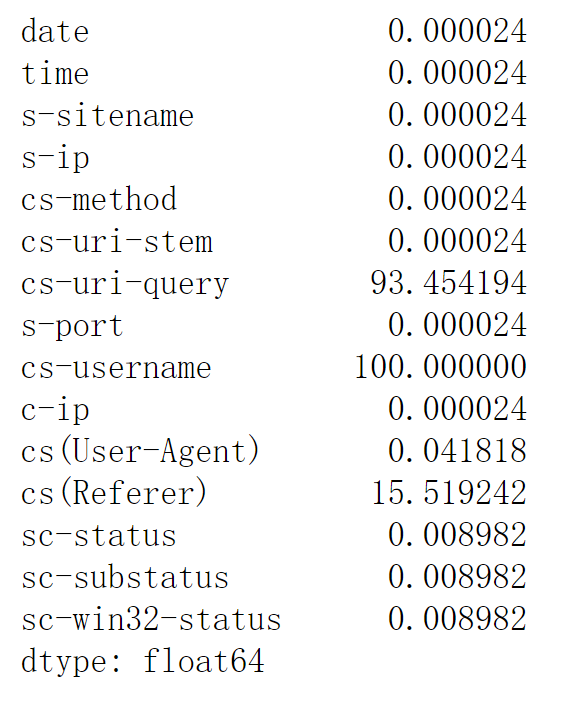
\includegraphics[width=0.6\textwidth]{Capture5.png}\\
	\caption{\DIFaddFL{loading}}\label{fig:loading}
\end{figure}
\DIFaddend 

\DIFdelbegin %DIFDELCMD < \blindtext
%DIFDELCMD < %%%
\DIFdelend \DIFaddbegin \section{\DIFadd{Data  visualization }}\label{sec-intro}
\DIFaddend 

\DIFdelbegin \section*{\DIFdel{Acknowledgement}}
%DIFAUXCMD
\DIFdelend \DIFaddbegin \begin{figure}
	\centering
	\selectcolormodel{rgb}
	%DIF > \missingfigure{Testing.}
	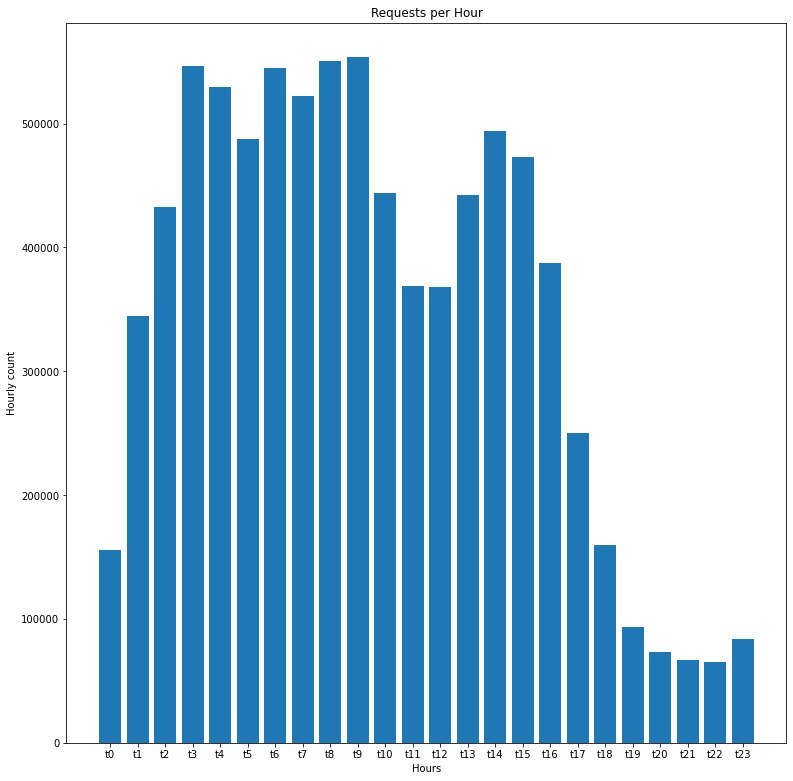
\includegraphics[width=0.6\textwidth]{ll1.png}\\
	\caption{\DIFaddFL{loading}}\label{fig:loading}
\end{figure}
\DIFadd{First of all, I analyzed the click traffic.
This is mainly for each hour to carry out statistics.
Speaking each hour the same row counts as the flow plotted out.
We can get some very interesting information. Due to the time difference, Melbourne time is adopted here, and we can see that there are more than 400,000 visitors in Melbourne time, and then there is a small peak from 2 to 9 in the morning, and then from 1 to 3 in the afternoon.
There are also fewer visits between 7pm and 11pm
}\DIFaddend 

\DIFdelbegin %DIFDELCMD < \lipsum[1]
%DIFDELCMD < %%%
\DIFdelend \DIFaddbegin \begin{figure}
	\centering
	\selectcolormodel{rgb}
	%DIF > \missingfigure{Testing.}
	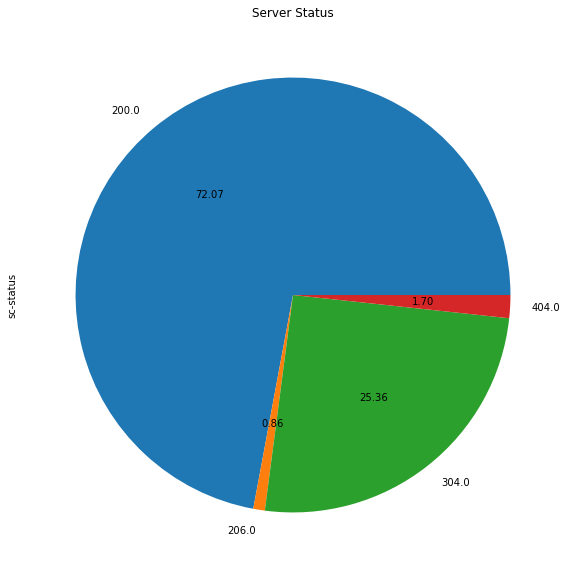
\includegraphics[width=0.4\textwidth]{ll2.png}\\
	\caption{\DIFaddFL{loading}}\label{fig:loading}
\end{figure}
\DIFadd{In the second step, I made statistics on the protocol status of the page visited by the user.
Six million people were the most successful.
In second place is rendering 304, which means the server has a cache for the web page.
This proves that the user has visited the site for the second or more times.
}\DIFaddend 


\DIFdelbegin \DIFdel{The authors would like to thank \ldots
}\DIFdelend \DIFaddbegin \twocolumn{
	\begin{figure}
		\centering
		\selectcolormodel{rgb}
		%\missingfigure{Testing.}
		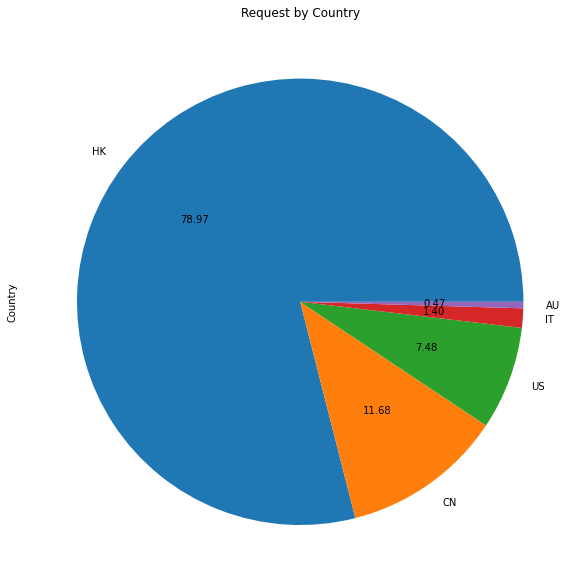
\includegraphics[width=0.6\textwidth]{ll3.png}\\
		\caption{loading}\label{fig:loading}
	\end{figure}
	The third step is to analyze the IP of users logging in the website, mainly from the perspective of country and city.
	You want to know the likelihood of a potential user's location.
	The first is the state.
	I found that Hong Kong, China and the United States are the top three countries to visit.
	Hong Kong is the majority, so re-marketing can focus on these three countries.
}{
	\begin{figure}
		\centering
		\selectcolormodel{rgb}
		%\missingfigure{Testing.}
		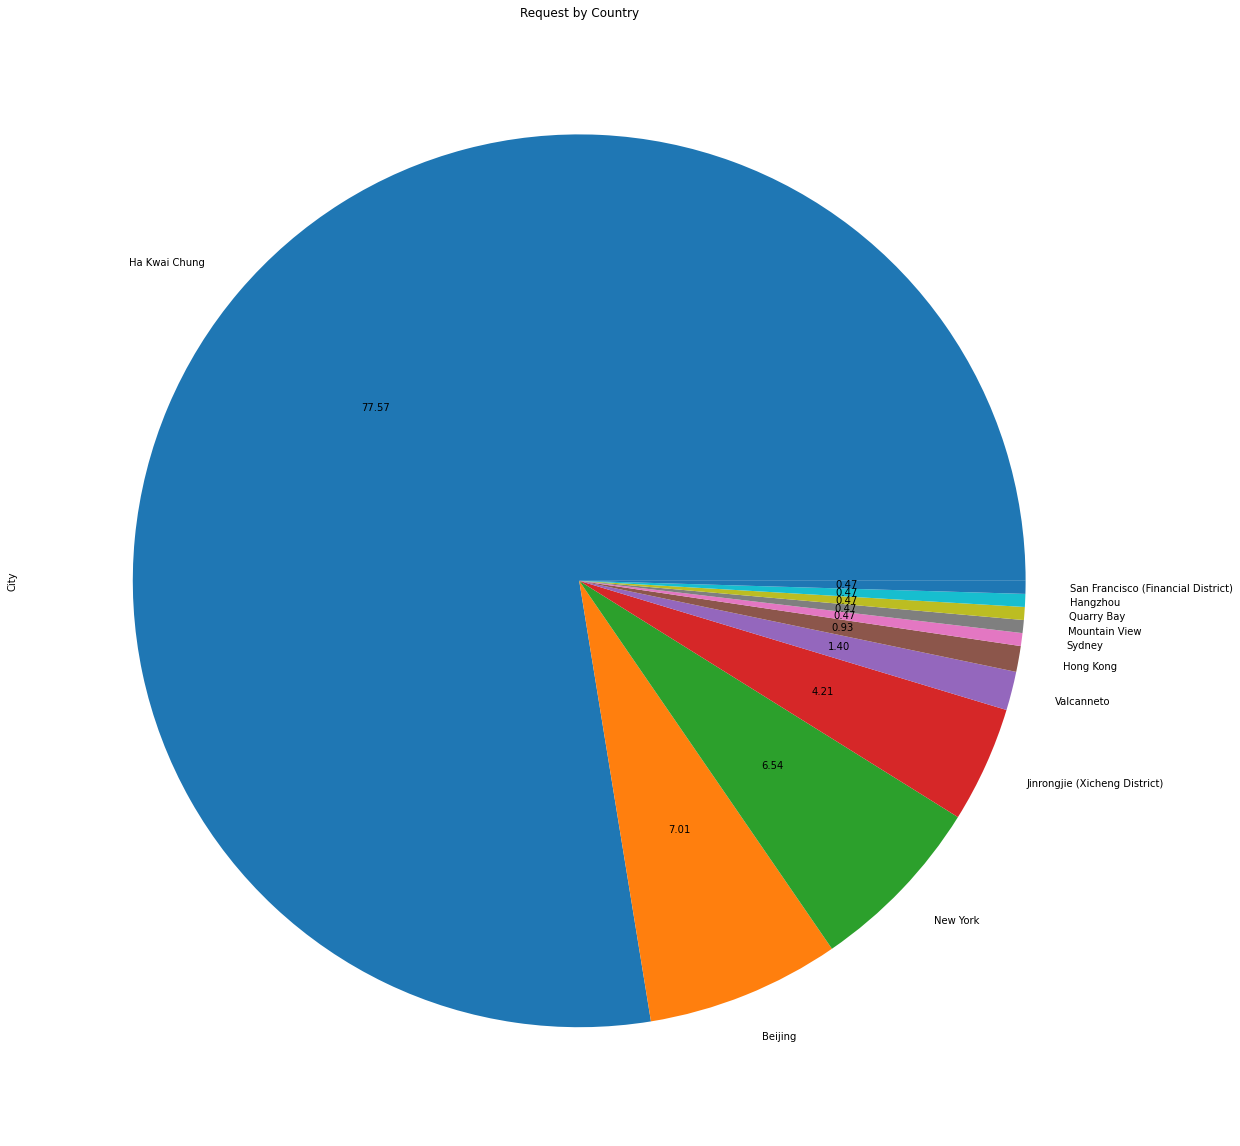
\includegraphics[width=0.6\textwidth]{ll4.png}\\
		\caption{loading}\label{fig:loading}
	\end{figure}

	when we look at the cities, we find that the first-tier cities of these three countries are the main visitors, such as Beijing in China and New York in the United States.
}
\DIFaddend 



%DIF <  ----------------------------------------------------------------
\DIFdelbegin %DIFDELCMD < \newpage
%DIFDELCMD < \bibliography{tuliplab,yourbib}
%DIFDELCMD < %%%
%DIF <  TODO: you should change this yourbib into a proper bib file name
%DIFDELCMD < \bibliographystyle{plainnat}
%DIFDELCMD < %%%
%DIF < =================================================================
%DIFDELCMD < 

%DIFDELCMD < \listoftodos
%DIFDELCMD < 

%DIFDELCMD <  %%%
\DIFdelend \DIFaddbegin \section{\DIFadd{Conclusions}} \label{sec-conclusions}
\DIFadd{So just to recap a little bit, the reason I did all four of these analyses was to try to understand how often people were visiting over that time period, how often they were visiting, whether they were first-time visitors or repeat visitors.
The main purpose of geographical analysis is to find out the geographical location of potential users, expand the market, and adjust the development strategy and planning of the organization in time.
 }\DIFaddend\end{document}

